%!TEX root = thesis.tex

\chapter{Related work}
\label{chap:rw}

\textit{[Section to be written.]}

\textit{[Content below copied from P2; to be adapted.]}

Many relevant research papers have been located and examined as part of the literature review stage of this project. Because my focus will be restricted to openly available Dutch geospatial datasets, I already know which sources of elevation measurements will be relevant. For reasons to do with the selection of available datasets and their accuracy-related characteristics (further discussed in Section \ref{sec:td} and Section \ref{sec:m}), my primary candidate is the national Lidar point cloud of The Netherlands, AHN. As a result, there are two main areas that are of interest in this literature review: Lidar accuracy (and derived DEM accuracy), and road feature reconstruction from Lidar point clouds. The literature review concerning these two areas will be presented below in separate subsections.

\section{Lidar accuracy}
\label{sec:lidaraccuracy}

\textit{[Section intro to be written.]}

\subsection{Accuracy description of Lidar sensing}
\label{sub:lidaraccuracy_sensing}

\textit{[Subsection to be written.]}

\textit{[Content below copied from P2; to be adapted.]}

\begin{wrapfigure}{r}{0.46\textwidth}
    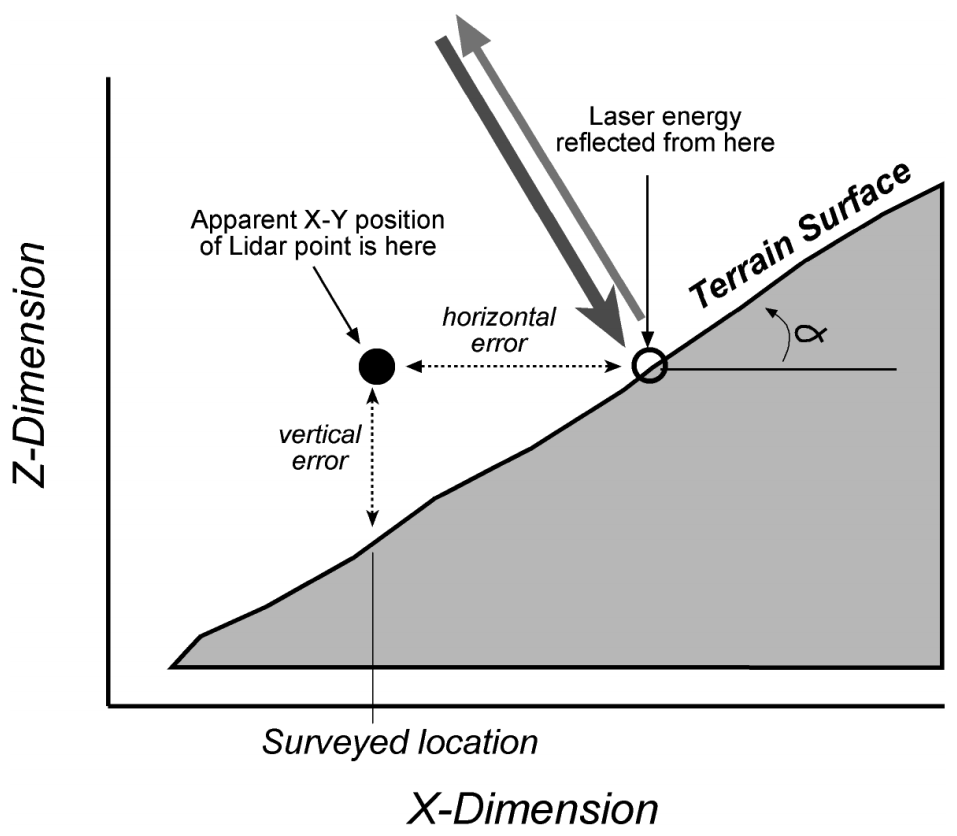
\includegraphics[width=0.95\linewidth]{final_report/figs/hodgson_breshanan_2004_01.png} 
    \caption{Sketch diagram showing the effects of horizontal error on vertical accuracy in the context of sloped surfaces. Any uncertainty in the lateral position of the point of reflection will be scaled by the tangent of the slope angle, denoted by $\alpha$ (\cite{hodgson_breshanan_2004}).}
    \label{fig:elevationaccuracy}
\end{wrapfigure}

Many papers describe that the accuracy of Lidar-derived DEMs depends on the accuracy of the sensing method itself. The notable paper \cite{hodgson_breshanan_2004} describes the most fundamental sensing errors of Lidar measurements to be introduced by Global Navigation Satellite System (GNSS, such as GPS) errors, Inertial Navigation Unit (INS) errors, Inertial Measurement Unit (IMU) errors, errors introduced by the waveform analysis algorithm and lastly, a general error factor that depends on the flying height. Combined, these are the primary factors that contribute to the measurement accuracy of a Lidar survey, together making up the nominal accuracy of a given survey, meaning the figures that can be found in the documentation accompanying Lidar data. It is shown by various papers including \cite{hodgson_breshanan_2004, su_bork_2006, kraus_etal_2006, raber_etal_2007, peng_shih_2006, chow_hodgson_2009, aguilar_etal_2005, aguilar_etal_2010, guo_etal_2010} that there are local factors influencing Lidar accuracy that are independent of the sensing equipment and are not generally reported in detail by data providers because they are difficult to estimate and vary spatially. This is not to say that are ignored by official figures entirely, for instance horizontal and vertical accuracy are reported separately by vendors because unlike horizontal accuracy, vertical accuracy also depends on the local terrain slope, as shown in Figure \ref{fig:elevationaccuracy}. It is widely regarded that the elevation error increases linearly as a function of increasing topographic complexity (commonly represented as a 2D slope map), and logarithmically as a function of decreasing local point density (falling off rapidly beyond a certain threshold density). Furthermore, an equivocal consensus also exists regarding the influence of vegetation. In all cases it decreases accuracy, with the significance of the error depending strongly on the type of vegetation. Mature trees and evergreens tend to influence accuracy to a lesser extent, whereas bushes, shrubs and undergrowth in general tend to have a decidedly larger impact. \cite{peng_shih_2006} quantified this as a function of \textit{vegetation angle}, a qualitative measure (not a real angle) that describes how well Lidar can theoretically penetrate various types of vegetation. They found that there is a linear correlation between elevation errors and vegetation angle, as well as canopy volume. The one exception is \cite{raber_etal_2007} which reported specifically that in very strongly vegetated areas, no correlation could be found between vegetation classes and accuracy (or even point density and accuracy). Research tackling these topics uses empirical methods to estimate errors, which generally consist of surveying ground control points accurately and either directly comparing with nearby Lidar points, or first constructing a spatially continuous DEM and comparing the interpolated values in the DEM with the surveyed reference elevations. The papers also establish that correlations exist between the examined sources of error, most importantly between vegetation and point density, with the latter intuitively decreasing in places of significant vegetation cover. Other correlations have also been reported, for instance between point spacing and vegetation angle, as well as point spacing and slope in \cite{peng_shih_2006}, and a weak logarithmic correlation between point density and slope by \cite{chow_hodgson_2009}.

The point is made in several of these papers that because of the logarithmic correlation between point spacing and accuracy, increasing the target point density of a survey is only justified up to a certain point. This depends strongly on the study area because point density itself is correlated with the vegetation cover and often the terrain relief. In most of the mentioned papers, the pinpointing of specific sources of error and the type of correlation include traditional methods of manual or automatic 1D or 2D regression, as well as for instance supervised classification with potential sources of errors as the variables. It is argued by several authors, most prominently by \cite{guo_etal_2010}, that in vegetation-free areas of low relief, most ALS surveys oversample the terrain by as much as 30 to 50 percent, leading to increased processing times, reduced algorithmic stability, and no improvement in accuracy. \cite{bater_coops_2009} comes to the same conclusion, and the logarithmic trend generally observed between point density and elevation accuracy further supports this. Conversely, in rugged, vegetation-covered terrain additional cross-flight surveys can increase accuracy significantly by improving ground point density, as \cite{peng_shih_2006} noted.

\subsection{Accuracy description of Lidar-based DEM-generation}
\label{sub:lidaraccuracy_dem}

\textit{[Subsection to be written.]}

\textit{[Content below copied from P2; to be adapted.]}

The topic of the influence of DEM interpolators (specifically, DTM interpolators) on accuracy has also been widely studied. There exist various types of approaches, such as deriving exact error propagation formulae from the mathematical descriptions of certain interpolators, as well as the more popular approaches based on simply performing the interpolation and checking its accuracy post-application via split-sample, cross-validation or jack-knife methods. As an example of the theoretical approach, \cite{aguilar_etal_2010} propagates errors mathematically through the IDW interpolator to obtain a specific expression. Among other things, such a formula depends on the sensing accuracy, the local factors of accuracy (e.g. slope), the gridding resolution, as well as a mathematical expression derived from the interpolator’s formal definition. As that paper shows, it is possible to simplify the process by performing Monte Carlo simulations on the mathematical definition of the interpolator rather than to derive the formula directly. \cite{kraus_etal_2006} also apply a similar, theoretical method to analyse errors propagating through the moving Maximum Likelihood Estimator (MLE). Post-application statistical evaluation was performed by for instance \cite{peng_shih_2006} (jack-knife, using surveyed reference points), and \cite{guo_etal_2010} (ten-fold cross-validation). Notably, \cite{smith_etal_2005} used all three approaches (split-sample, cross-validation, and jack-knife) for a wide range of interpolators in an urban setting.
Firstly, many of these papers examined the influence of gridded DTM resolution on accuracy. \cite{chow_hodgson_2009} examined via regression techniques (on IDW interpolation) how it is correlated with point density and found that linear to logarithmic correlations exist. \cite{guo_etal_2010} argues that for most interpolators, the overall trend is linear between accuracy and resolution, up to the scale of the Lidar point density. They also found that differences in accuracy between interpolators were most prominent at the finest resolution. \cite{bater_coops_2009} found that the local influence on accuracy of slope and point density are mostly invariant relative to DTM resolution. In terms of the accuracy ranking of interpolators, there is a clear consensus that no such ranking exists that is independent of the size and type of the study area, and the purpose of the interpolation. For instance, the accuracy of piecewise spline-based, quintic-type, kriging and ANUDEM methods were found lacking in the context of their insensitivity to small, sudden changes (such as natural faults in the terrain and anthropogenic modifications thereof) while they were proven to work well for large-scale terrain, as described by \cite{bater_coops_2009} and \cite{guo_etal_2010} for instance. All reviewed papers agreed that the accuracy of all interpolators decreases the most in areas of high relief and reduced point density, with spline-based, IDW methods generally producing the worst results in such areas, especially for large-scale terrain. Interestingly, the relative importance of interpolation-introduced errors is reportedly low relative to instrument-related errors and surface-related local sources of error, according to research such as \cite{hodgson_breshanan_2004} and \cite{aguilar_etal_2010}. The former goes as far as to state that the decrease in accuracy after the application of an interpolator is insignificant, or that interpolation may even increase the overall accuracy, although this was observed in densely vegetated areas where point spacing and accuracy are severely afflicted. TIN-based interpolation methods were recommended specifically by \cite{bater_coops_2009} for complex geometries and found it in their research to be the most conservative in terms of RMSE analysis. \cite{hodgson_breshanan_2004} also used TIN-based interpolation in their research, and detected no significant decrease in accuracy following interpolation. Furthermore, \cite{peng_shih_2006} used TIN-based interpolation in their research, in which they found local influences on elevation accuracy highly predictable. Unlike most papers, \cite{aguilar_etal_2010} considers the accuracy of ground filtering explicitly, and states that its success is a precondition of accurate terrain interpolation wherever the terrain is occluded or shaded partially. It suggests the estimation of ground filtering error (even if only from generic values) and its inclusion in overall elevation accuracy. Overall, it is evident from the review (and specifically recommended by various authors) that testing several candidate interpolators before making a final choice is recommended.

\section{Road identification in point clouds}
\label{sec:roadidentification}

\textit{[Section intro to be written.]}

\textit{[Content below copied from P2; to be adapted.]}

Our second domain of interest is feature extraction because our intention is to not only systematically query a DEM for elevations around the NWB road centrelines, but to take into account the entire road surface as represented by the point cloud. This requires one to identify, or at least approximate which point cloud points were reflected from the surface of the given road.

\subsection{Research using point clouds only}
\label{sub:roadidentification_pconly}

\textit{[Subsection to be written.]}

\textit{[Content below copied from P2; to be adapted.]}

In terms of point cloud feature extraction techniques relevant to roads, I have looked at a range of papers that give account of a spectrum of divergent methods. One strategy, most prominently represented by \cite{hu_2003, hu_etal_2004, zhu_mordohai_2009, zhu_hyppa_2014, lin_etal_2015}, is based on the idea of transitioning to a photogrammetric analysis at some point in the process. First, a set of pre-processing techniques to better characterise potential road points in the source Lidar data are applied, generally by performing some form of filtering (in some cases simply by setting thresholds applicable to returns from bitumen), or by extracting ground planes using various techniques and selecting points that lie close to them. Then, images are rendered from the point cloud from various angles, often using colour-coding based on point properties, and applying photogrammetric methods to identify roads. Sometimes high-definition aerial or satellite imagery is incorporated in the photogrammetric workflows. The success rates of such strategies are mediocre, rely strongly on manual parametrisation, and are unsuitable for large study areas with inhomogeneous types and distribution of roads, as also concluded by the literature review in the paper \cite{yang_etal_2013}.

A further popular set of strategies rely on road curb detection. \cite{vosselman_zhou_2009}, \cite{zhang_2010}, and \cite{yang_etal_2013} are examples of such research. \cite{vosselman_zhou_2009} presents a method in which a DTM is generated, points close to it are selected in the point cloud, and small, curb-like jumps in elevation are algorithmically detected. The curb points are selected, and a feature extraction method (RANSAC in this case) is used to construct 3D lines from them. Gaps in the lines are closed algorithmically, and B-splines are fitted to optimise the shapes of the road edges. In \cite{zhang_2010}, road cross-sections are inspected in 1D, and the points representing the road surface, the curbs and non-road surfaces are identified. In \cite{yang_etal_2013} an approach is presented in which first cross-sections are identified, ground points are filtered in 1D, and curbs are then identified in the 1D series of ground points.

\begin{wrapfigure}{l}{0.5\textwidth}
    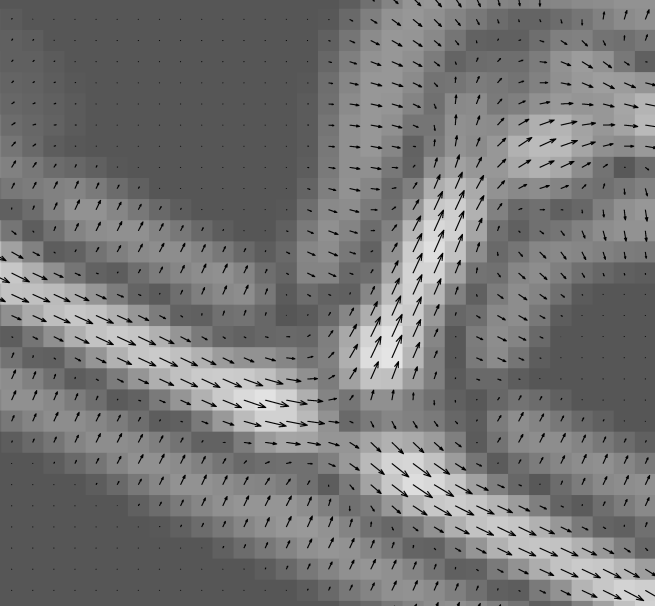
\includegraphics[width=\linewidth]{final_report/figs/clode_etal_2007_01.png} 
    \caption{Illustration of the results of PCD convolution. The vector magnitude in any given pixel quantifies the support that exists there for the presence of a road centreline, so it is effectively a centreline detector (\cite{clode_etal_2007}).}
    \label{fig:phasecodeddisk}
\end{wrapfigure}

Their approach is unique because it uses moving window (i.e. convolution) methods on the 1D sections to extract the curbs, testing a subset of the points in each iteration to see whether they satisfy a range of rules. While the results of these methods are more flexible, more accurate and more complete in general than the photogrammetric methods, they are not, in their original form, well suited for this project. The cross-section based approach was originally developed for MLS data, where the data is either natively output in the form of road cross-sections (car-mounted front facing sensor), or can be easily extracted from the point cloud in such a form.

The work \cite{vosselman_zhou_2009} is an exception, which demonstrates that a relatively simple approach can be used to detect curbs without the need for native cross-sections in the data. However, a deeper issue undermines our confidence in the applicability of curb-detection methods. Working with a national dataset and focusing on large roads (including motorways) means that the assumption that well-defined, relatively uniform road curbs will exist and be reliably detectable everywhere is not a sensible assumption.

There are many more papers dealing with this task without using external vector data. For instance, \cite{clode_etal_2004} and \cite{clode_etal_2007} present a set of methods in which first a DEM is generated, then points close to the DTM are selected, are further filtered based on intensity thresholds applicable to bitumen in a hierarchical system, and then the results are refined via morphological operations on the selected regions. The output is a point cloud in which road points are marked semantically as belonging to a road. In the 2007 paper, they extended the procedure by convolving the results with a Phase Coded Disk (PCD), which can create a spatial map of the predicted road parameters wherever it moves through road points. Convolving the PCD is in fact a photogrammetric method, because it acts on a raster generated from the classified point cloud prior to its application. Nevertheless, the method is still more relevant to us than the rest of the photogrammetry-based research mentioned here. An example visualisation of its output is shown in Figure \ref{fig:phasecodeddisk}. They describe it as an alternative to using the Hough-transform for finding road centrelines, which, according to their research, is not reliable enough in this context. This spatial map can then be used to generate a vector dataset describing the geometry of the roads.

\cite{gross_thoennessen_2006} shows that point neighbourhood information can be used to generate covariance matrices of individual points, which can in turn be used to decide directly whether the point belongs to a linear feature. They also describe how lines can be assembled from the selected points efficiently. Other methods relying only on the points themselves exist, but they are typical of real-time MLS applications, such as the fully convolutional neural network-based solution in \cite{caltagirone_etal_2017}. The literature review in \cite{yang_etal_2013} offers an excellent overview of such additional methods, but they will not be described here any further, as they are not relevant enough to this project.

\begin{figure}[h]
    \centering
    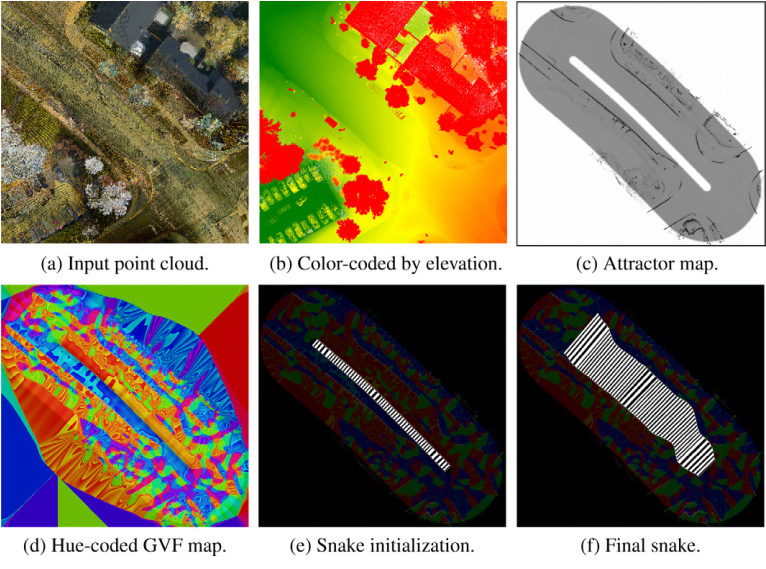
\includegraphics[width=0.75\linewidth]{final_report/figs/boyko_funkahuser_2011_01.png} 
    \caption{Illustration of the procedure used in \cite{boyko_funkhauser_2011}, taken from their paper. In the attractor map, darker colours represent stronger attraction, resulting in the active contour converging to them in the optimisation procedure. The GVF map is a vector map that contributes to favourable active contour convergence and is not described any further here. The initial contour is based on the road centreline (from external vector data).}
    \label{fig:activecontouroptimisation}
\end{figure}

\subsection{Methods using input point clouds and external vector data}
\label{sub:lidaraccuracy_external}

\textit{[Subsection to be written.]}

\textit{[Content below copied from P2; to be adapted.]}

This last category contains research that used similar input data to mine (including initial road estimate vector datasets) and achieved similar goals.

\cite{cai_rasdorf_2008} show that enriching road centrelines with elevations can be achieved using simplistic methods. Their first method is based on finding points on opposite sides of roads (in 2D) at similar distances from them, and in suitable locations to form approximate cross-sections. Roads are intersected with the cross-section and the intersections are given elevations by 1D-interpolating inside the cross-sections, using the elevations of the two points defining them. Their second method is even simpler; for each road vertex  (or some sampling along its length), they locate the closest Lidar point and associate its elevation with it. The simplicity of these methods is reminiscent of the commercial solution which were developed for NDW by RHDHV (described in Section \ref{sec:m}), and highlights that a rough approximation for the road elevations can, in practice, be made either directly from the point cloud or from a derived DTM in a straightforward manner. However, far more sophisticated methods have been developed by other authors.

One landmark research, \cite{boyko_funkhauser_2011}, describes a method in which their input polylines are used to label road points in an ALS point cloud. They first associate the input lines with elevations by fitting spline curves through nearby Lidar points. Suitable Lidar points are selected based on minimising an error function that includes terms related to the distance from the location of interpolation, and to elevation variance. The resulting network is guaranteed to be continuous and smooth because the densified input polylines are used as a spline control points. They then partition the point cloud on disk, based on fitting small support planes along the 3D-converted lines and fetching points that are close to them (solving both the memory and the 2.5D violations related to overlapping roads). They then construct a map penalising points away from road edges based on one term depending on the distance from the road centreline, and another based on a curb detection algorithm (these are so-called \textit{attractor maps}). Lastly, they apply an active contour (snake) optimisation technique that yields the road edges in 3D, and then label points between the two edges as road points. An illustration is shown in Figure \ref{fig:activecontouroptimisation}.

\begin{wrapfigure}{r}{0.5\textwidth}
    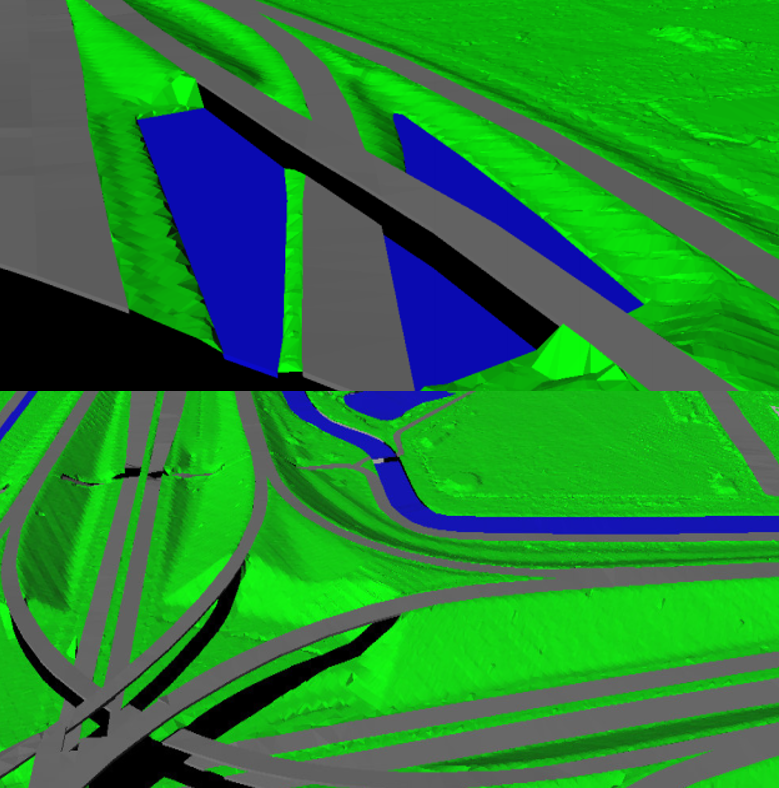
\includegraphics[width=\linewidth]{final_report/figs/oudeElberink_vosselman_2006_03.png} 
    \caption{Examples of 3D-converted multi-level road vector geometry showing artefacts that are typical in the context of Lidar point cloud to 3D vector geometry conversion. Most notably, in multi-level configurations of roads, only the one with the highest elevation is converted to 3D (\cite{oudeElberink_vosselman_2006}).}
    \label{fig:conversionartefacts}
\end{wrapfigure}

In the research \cite{gopfert_etal_2011} it was demonstrated that such active contours can be used to estimate road outlines without the need for the involved pre-processing steps of \cite{boyko_funkhauser_2011}, simply by taking elevations of the input polylines from a derived DTM and optimising the road centreline the same way as its outline (using the active contours).

The work \cite{hatger_brenner_2003} presents two approaches based on region-growing. The first one is based on growing planes in the entire study area from Lidar points. This being too complex computationally, they propose another approach of treating Lidar scan lines individually, partitioning each into parametrised line segments via linear regression and then inspecting the succession of scan lines and identifying neighbouring segments that are roughly parallel. The resulting groups of (roughly parallel) lines are then treated as planar regions, and an additional region growing step is performed to find any points that might have been left out. The results of this can then either be prepared as a full, 3D-polygon-based planar partition of the study area onto which road polylines can simply be projected, or by further refining the planar partition (eliminating small, meaningless planes) via a RANSAC-based workflow.

The work \cite{oudeElberink_vosselman_2006} is relevant not only because of the methods it applies, but also the datasets. They enrich the best-known Dutch open data national topographical vector dataset (the present-day equivalent of which is BGT) with elevations, and as their source of elevations, they use AHN data.

They do not exclusively consider roads; all polygonal vector objects are extruded to 3D. Like \cite{hatger_brenner_2003}, they propose region growing as the foundation of the elevation extraction workflow. They use the Hough transform to find seed points whose neighbourhood suggest a planar structure, fit planes and then grow by checking the point-to-plane distance of new points, labelling points with the identifier of the plane they belong to. The vector data is then overlaid, and for each polygon the plane is selected which is represented by the most labelled points in its interior. These points are re-fitted a plane, and each such plane is used to extrude the corresponding overlaid vector geometry simply by projecting onto its surface. To improve upon the results of this simple extrusion, they suggest the application of algorithmic topological corrections. Furthermore, to model the interior of the extruded polygons in more detail, they recommend the construction of a Constrained Delaunay Triangulation (CDT) for each, first by inserting its edges as constraints, and the by inserting the Lidar points that generated its surface. The CDT can be refined algorithmically to ensure smoothness. The main limitation of their method is that its method to extract elevations (the region growing approach) is not too accurate, and that it cannot handle overlapping objects, such as roads in motorway interchanges. Some typical artefacts are shown in \ref{fig:conversionartefacts}.

Their method was later extended in \cite{oudeElberink_vosselman_2009} to work well in complex multi-level road settings by using point cloud segmentation in a manner resembling what I already described in the context of \cite{boyko_funkhauser_2011}. In his doctoral thesis \cite{oudeElberink_2010} he combined this method with the overall procedure in \cite{oudeElberink_vosselman_2006} to form one integral whole. Furthermore he extended it with a road extraction quality assessment procedure, which was later perfected and also published separately in \cite{oudeElberink_vosselman_2012}. Their quality and accuracy assessment methodology is comprised of two separate procedures and the comparison of their results: a theoretical (functional and stochastic) evaluation, and an empirical one against reference data. Interestingly, their reference data was DTB (see Section \ref{sec:td}) and in general, showed good agreement with their road extraction results.

\section{Summary of literature review}
\label{sec:rwsummary}

\textit{[Section to be written.]}

\textit{[Content below copied from P2; to be adapted.]}

While none of the above research provides an all-in-one solution to answering the research questions of this project, they contain procedures and concepts which can be used as building blocks for my methodology. The main area \textit{not} explicitly covered by the examined papers is the use of external 3D vector data (DTB in our case) as a further constraint when extracting roads from point clouds. However, methods to perform this can be derived from the operations in them that relate to using vector geometries as approximate road locations in 2D, and from general geomatics concepts and methods. An additional consideration related to the input road centrelines is that in all research presented above, refining the lateral position of the road is permitted. However, NDW specifically requested that I do not move the NWB lines horizontally. Hence, I plan to focus primarily on enriching NWB with elevations without moving them laterally, with only exploring its lateral refinement to a limited extent.

\section{Input assessment}
\label{sec:input}

In terms of datasets, both the commercial implementation and the proposed research rely on the following three sources:

\begin{itemize}
\item Nationaal Wegenbestand (NWB, National Road Database)
\item Actueel Hoogtebestand Nederland (AHN, Current Dutch Elevation)
\item Digitaal Topografisch Bestand (DTB, Digital Topographic Database)
\end{itemize}

As mentioned in the section about research questions, I am also planning to examine how specific datasets from individual NDW data suppliers (such as municipalities, road authorities, civil engineering agencies) can be integrated in the procedure and how they affect the accuracy. At this stage in the project, the specific datasets have not been selected yet.

\subsection{Nationaal Wegenbestand – NWB}
\label{sub:nwb}

\textit{[Subsection to be written.]}

\textit{[Content below copied from P2; to be adapted.]}

\begin{figure}[h]
    \centering
    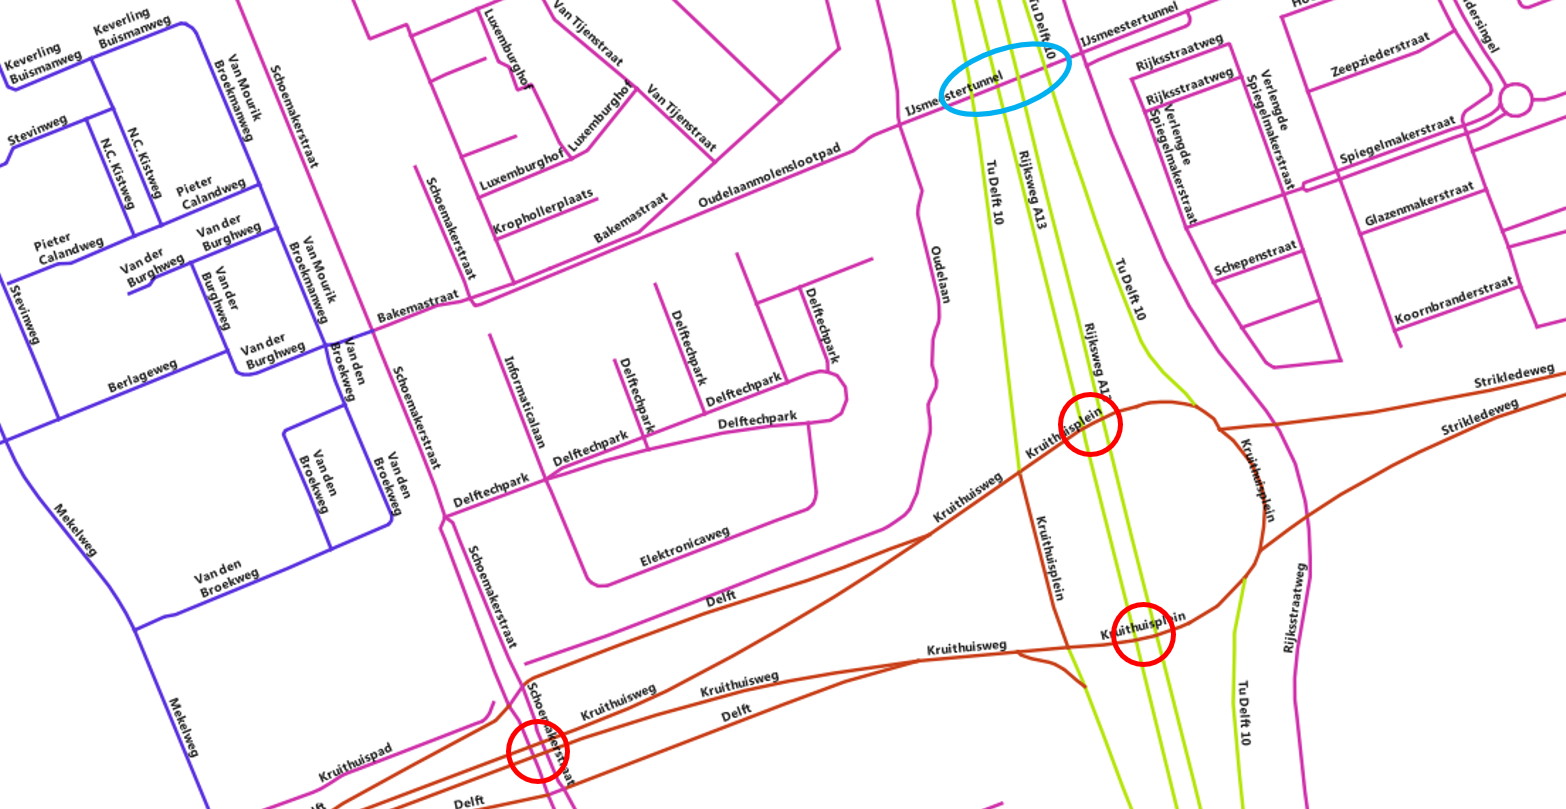
\includegraphics[width=\linewidth]{final_report/figs/nwb_sample_02.png} 
    \caption{An example render of NWB. The road segments \textit{(wegvakken)} are colour-coded to indicate management \textit{(wegbeheerdersoort)}. Yellow is used for R-roads (state-managed roads), red denotes P-roads (province-managed roads), magenta means G-roads (municipality-managed roads), and W-roads (RWS-managed roads) are not shown in this figure. Blue roads (T-roads) are roads which do not fall into the above 4 categories, in this case they are managed by TU Delft. This render also contains examples of challenging 3D relationships. Where the P-road Kruithuisweg/Kruithuisplein crosses the G-road Schoemakerstraat and the R-road A13, no intersection occurs in 2D because the roads cross over one another in 3D. These locations are indicated in the figure by red circles. Furthermore, where the bike path IJsmeestertunnel (a G-road in NWB) crosses the A13, a series of 3 short tunnels are located in reality. This is indicated in the figure by a blue oval. These are two types of road layouts that we expect to have to dedicate special attention to.}
    \label{fig:nwb}
\end{figure}

NWB (or more specifically, NWB-Wegen, the NWB roads product) is an \textit{ESRI Shapefile}-based vector dataset comprised of a semantically rich set of 2D \textit{MultiLineString} objects. They are interconnected in such a way that NWB can be regarded topologically as a graph representation of the Dutch road network. Although the NWB contains all named and numbered roads in The Netherlands, we are only interested in roads that are semantically marked as state-owned or province-owned (category R for Rijk and P for Provincie), because the new noise regulation is only relevant to these types. NWB and the road types it contains are illustrated in Figure \ref{fig:nwb}. In addition to its important topological graph structure, the NWB lines are georeferenced with good accuracy. Although the accurate nature of its georeferencing is specifically mentioned in the documentation of the data, it is not evidenced by a rigorous evaluation. The quality description includes only a single figure, which is 5-metre accuracy at two standard deviations (i.e. 95\% confidence), but with the confidence being based on the total number of roads, implying that the accuracy evaluation method is performed on a road-to-road basis, each of which may be comprised of multiple \textit{MultiLineString} objects. It is not described, how the accuracy is evaluated for each road, for instance whether it is based on the accuracy of the vertex locations of the road, an arbitrary sampling along their length, and how it is aggregated. Furthermore, we do not know whether the reference for the accuracy was empirical (surveyed control points) or whether it is purely theoretical and is based on the sources and the methods involved in creating  and updating the dataset. Both the topological and the geographical information content of NWB is assembled from a wide range of providers ranging from large national providers such as RWS and Kadaster, to local providers such as specific road authorities and civil engineering agencies. No clear indication is given in the documentation about the sources used for the compilation of specific NWB road types or the estimation of their accuracies, but it is mentioned that they are inconsistent across the range of road types (\cite{nwb_docs}). Although the above nominal lateral accuracy (and its description) is not sufficient for compliance with the new noise regulations, the 3D conversion of NWB is not concerned with improving it – in fact, it is a requirement of the project not to displace NWB horizontally. Hence, we may say that the intended outcome of the 3D conversion is to devise a method that can produce accurate elevations for NWB assuming it  is up to SWUNG2 standards. To achieve this in practice, lateral refinement is being done in a separate project by developing a workflow to match NWB roads with roads in another Dutch national open data geospatial dataset called Basisregistratie Grootschalige Topografie (BGT). Since BGT is already compliant with the accuracy requirements, correcting NWB geometries based on BGT will foreseeably solve the lateral accuracy problem of NWB. However, at the time of writing of this report, the BGT-based correction has only been carried out and released for municipality-owned roads (category G for Gemeente), hence both the commercial and the scientific 3D-NWB project still rely on NWB data that lacks this correction (\cite{nwb_gecorrigeerd}). Regardless of improving NWB’s lateral accuracy not being within the scope of this project, it is important to be aware of the uncertainty because of its implications when overlaying NWB with other datasets, such as AHN and DTB.

\begin{figure}[ht]
    \centering
    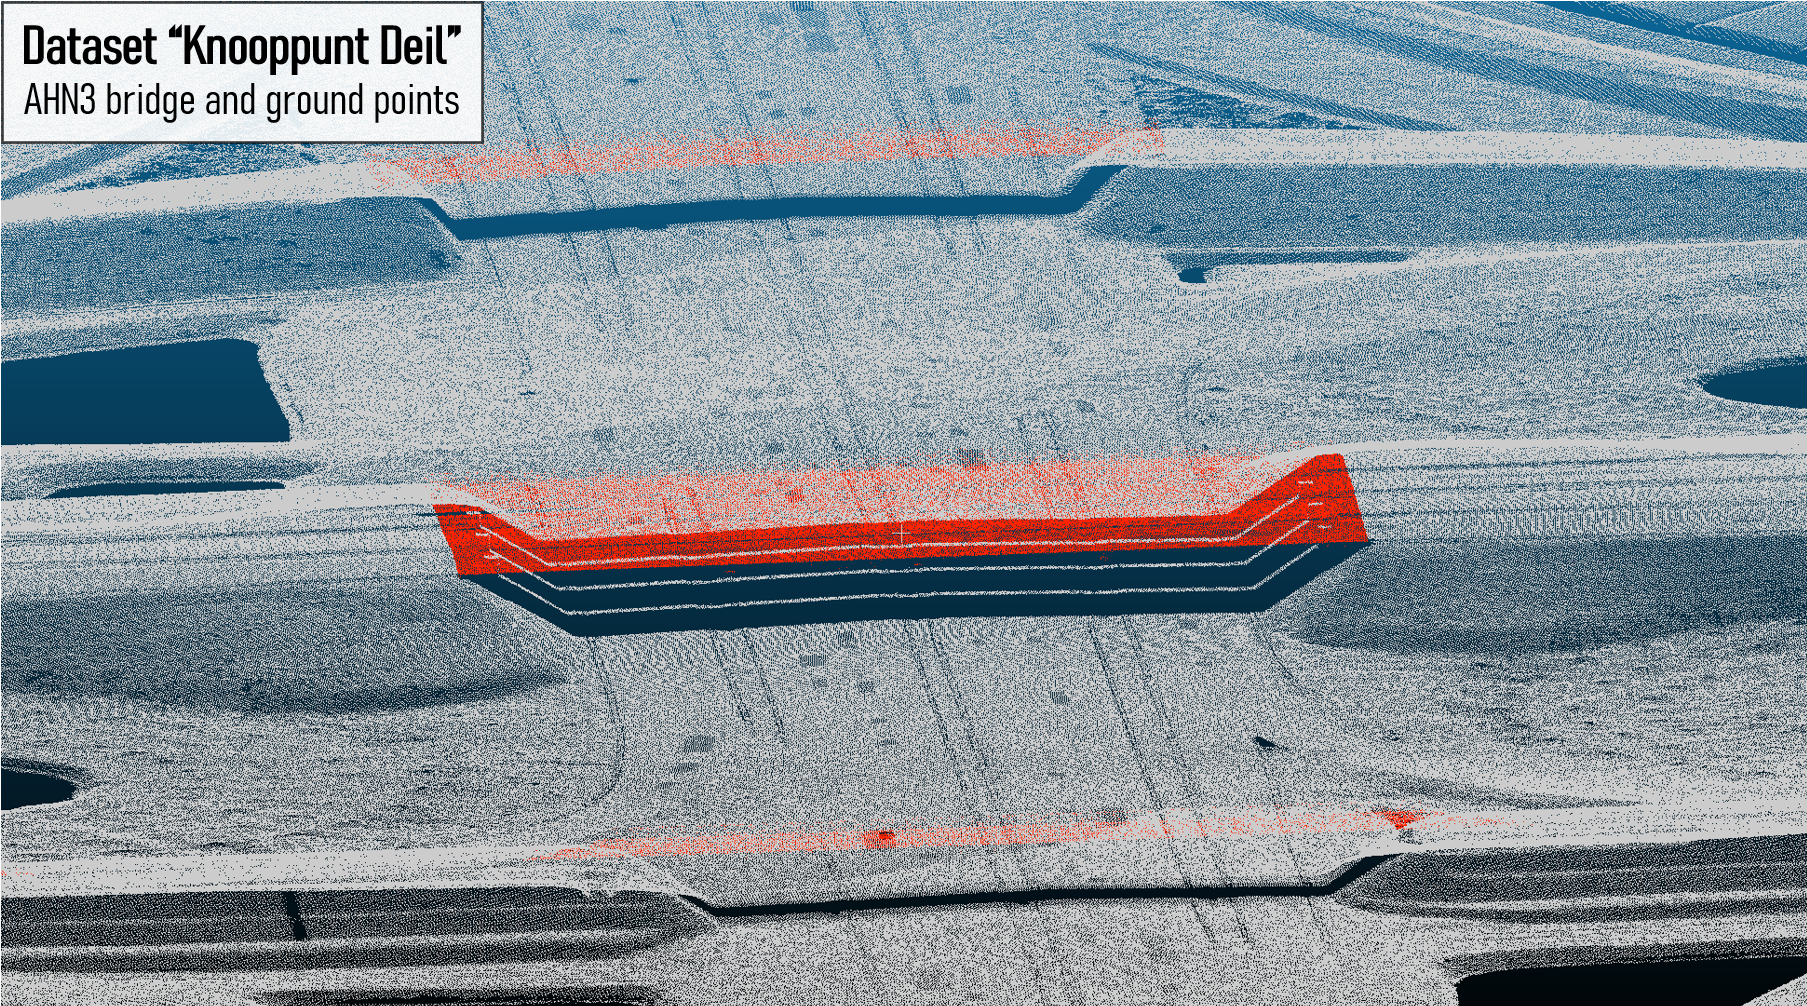
\includegraphics[width=\linewidth]{final_report/figs/ahn_sample_01.png} 
    \caption{An example render of AHN3 with the original point density (no thinning applied) at the Knoppunt Deil, SW of Geldermalsen. The white colour corresponds to ground points (class 2), red corresponds to bridges (class 26). All other classes were removed. The shapes of motorway lanes and ramps, as well as bridges are clearly defined. Road constructed on elevated ground is reliably classified as ground, bridges are cleanly split off by the classification. Even under thin bridges, data becomes gradually sparser at the border and becomes extinct directly below the bridge. This render also makes it clear that wherever vehicles were encountered, the sampling is worse locally. It does not go entirely extinct however, as most locations have been scanned multiple times.}
    \label{fig:ahnbridges}
\end{figure}

\subsection{Actueel Hoogtebestand Nederland – AHN}
\label{sub:ahn}

\textit{[Subsection to be written.]}

\textit{[Content below copied from P2; to be adapted.]}

AHN are airborne Lidar (ALS) survey datasets available as open government geospatial data in The Netherlands. The surveys are commissioned every few years with AHN1 to AHN3 already complete (1996 to 2019), and the first AHN4 surveys nearing release. At this stage of the project, we are interested in AHN3, although it is a planned side-track of the research to examine how freshly released AHN4 data could best be made use of. The dataset has a combined systematic and stochastic elevation error of 15 centimetres at two standard deviations (i.e. 95 \% confidence), and 6 to 10 points per square metre point density on average, corresponding to a 0.41 to 0.32 metre posting distance. The lateral error is 18 centimetres at two standard deviations (\cite{ahn_kwaliteit}). Comparing these to the descriptors of datasets mentioned in research examined as part of our literature review (see the Relevant work section), AHN3 can be considered accurate, and to have excellent point density. The AHN3 point cloud has been classified semi-automatically with great accuracy and is released with the classification included. This means that for most purposes, the point cloud needs not be ground filtered manually, and that extracting certain features is made far easier. Of the various classes available, we are interested in class 2 the most, which corresponds to ground points, and class 26 which contains, among other things, bridges. Ground points are primarily interesting to us because they contain the road points. This includes roads that were constructed directly on the terrain, as well as roads constructed on altered terrain, such as those built on elevated ground or in open trenches. It also contains the points that represent the terrain in the vicinity of the roads. Elevated roads and bridges are not considered ground points and are generally represented by gaps in class 2, which can, in most cases, be filled by using data from class 26, as shown in Figure \ref{fig:ahnbridges}. However, it is worth noting that class 26 also contains other types of objects, for instance large motorway signs arching over the road surface (shown in Figure \ref{fig:ahnsigns}), as well as the civil engineering structures of elevated roads and bridges (in addition to the road surfaces on them).
\begin{figure}[h!]
    \centering
    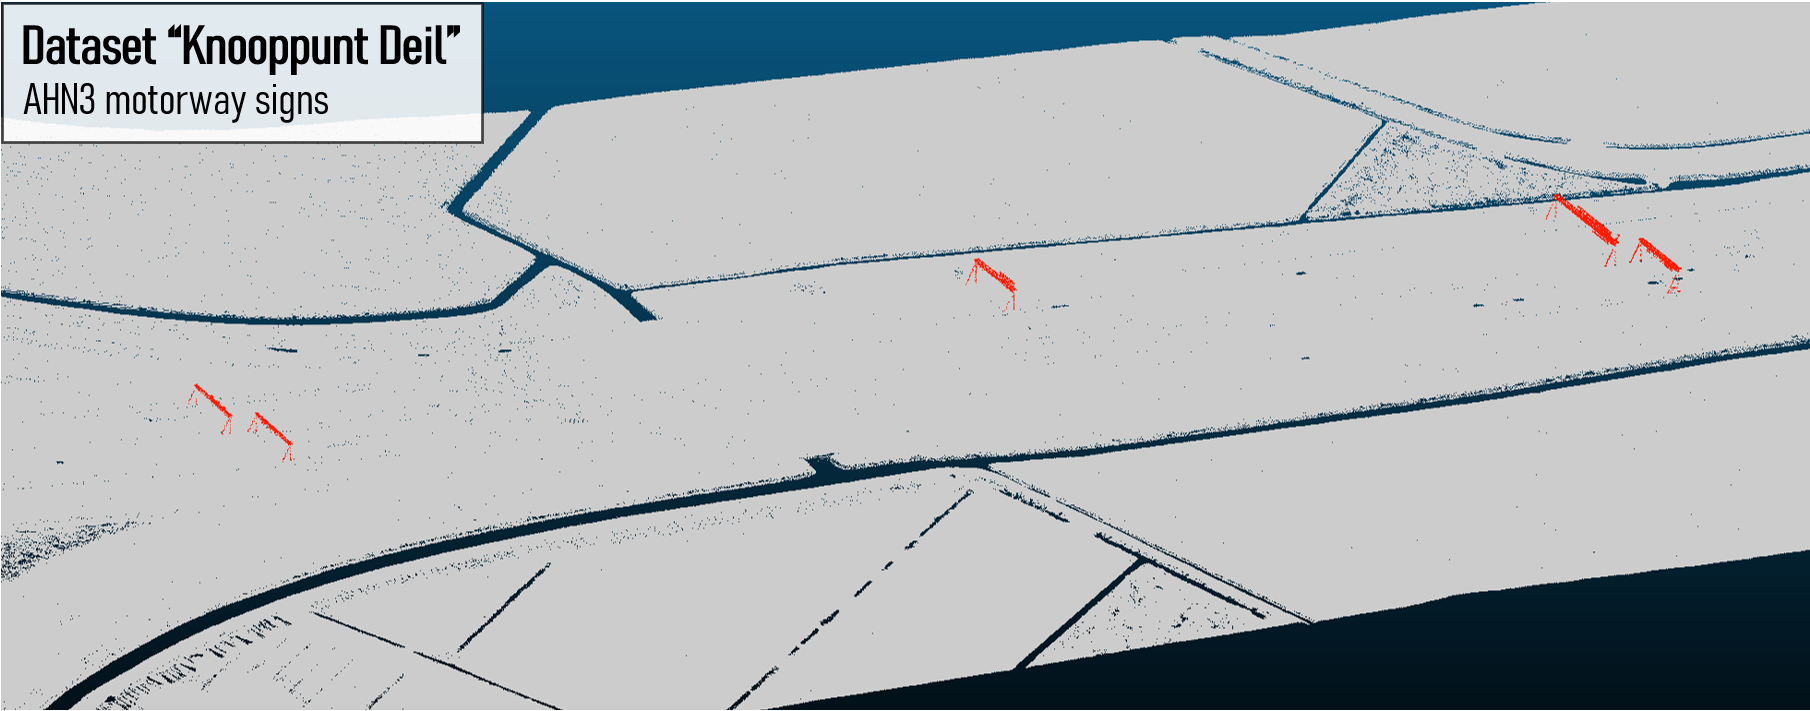
\includegraphics[width=\linewidth]{final_report/figs/ahn_sample_02.png} 
    \caption{This render is from the same location and data as \ref{fig:ahnbridges}. Here it is visible that my testing datasets, all points falling outside a 150-metre buffer zone around the NWB centrelines have been removed. While class 26 primarily contains bridges, this image shows that full-width motorway signs are also contained by it. It also shows that the presence of water results in holes (the dark, linear features running parallel with the motorway in this render) in the ground-only point cloud.}
    \label{fig:ahnsigns}
\end{figure}
\begin{figure}[h!]
    \centering
    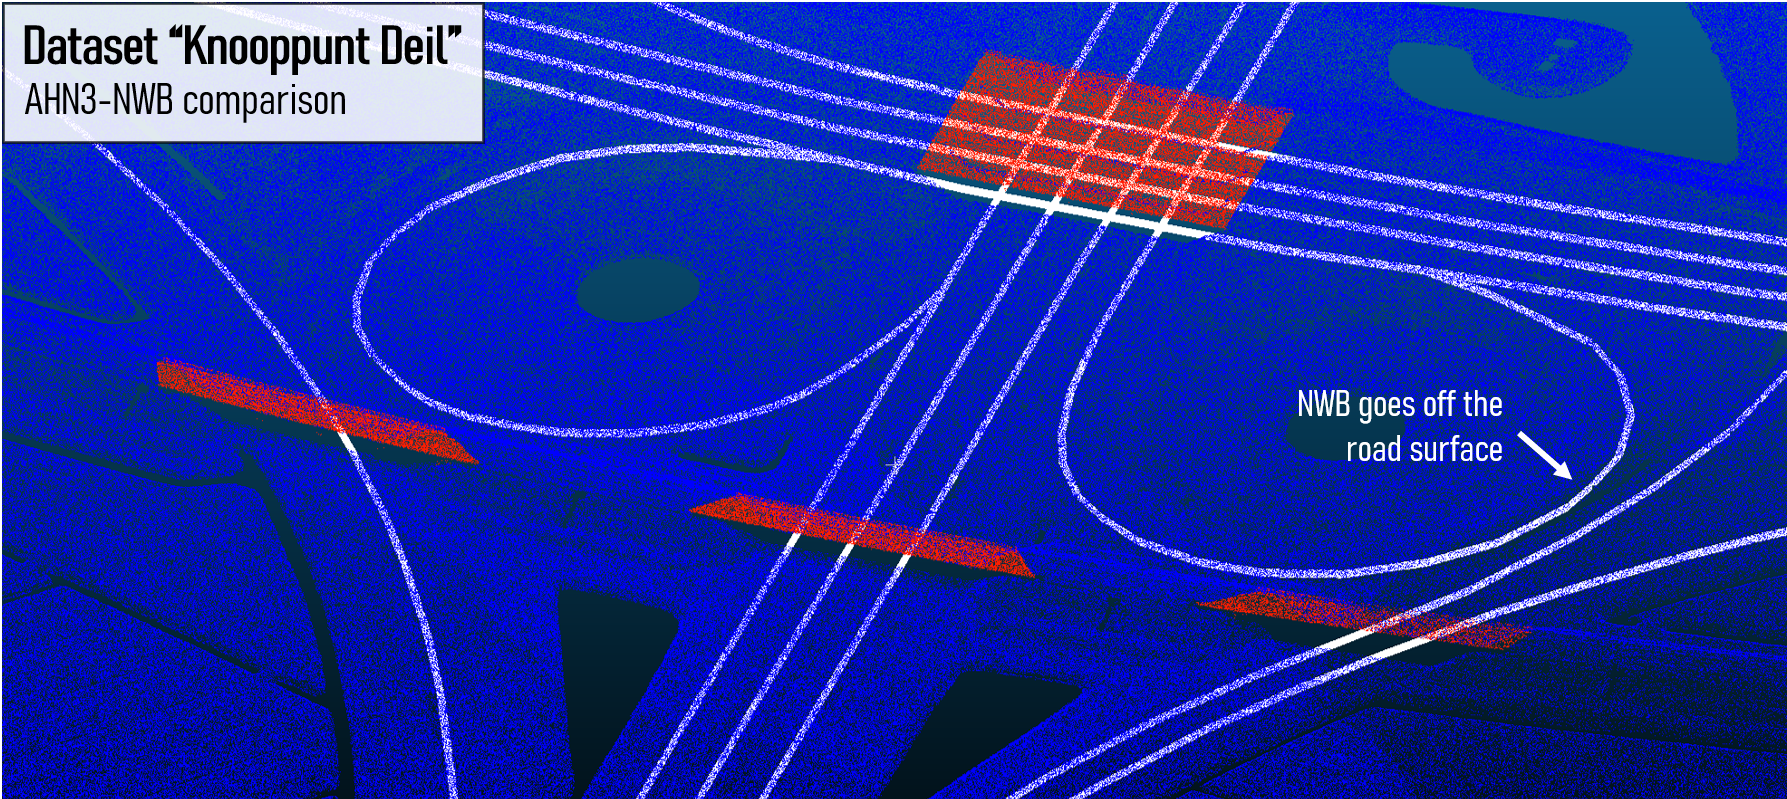
\includegraphics[width=\linewidth]{final_report/figs/ahn_sample_04_a.png} 
    \caption{This render is from the same location and data as Figures \ref{fig:ahnbridges} and \ref{fig:ahnsigns}. Here, ground points are coloured blue, and NWB centrelines are shown in white. As they have no elevation, they appear below AHN3 points and are consequently masked out partially by them. In general, the visual agreement between AHN3 and NWB appears to be good. The most noticeable deviations from the AHN3-defined centrelines of roads occur where they are intensely curved, and where motorway ramps merge into motorway lanes. The reason for the prior appears to mostly be the angularity introduced by the finite discretisation of curves in NWB, for instance in the location pointed out by the green arrow. The succession on three bridges in the bottom of the image do not have an associated NWB centreline because they are railway bridges. The same would be observed for roads not yet registered in NWB (i.e. newly roads).}
    \label{fig:ahnnwb}
\end{figure}
AHN3 is released in the form of a point cloud, as well as DSM and DTM rasters. Both DEMs were produced using basic radial IDW interpolation with a fixed parametrisation. The DTM was generated by including only points from class 2 in the interpolation step. They are available at 0.5-metre and 5-metre resolutions, with the 0.5-metre resolution being relevant to this project in terms of the target accuracy. For context, this raster converts (on average) 1.5 to 2.5 points into a single raster cell. The Lidar tiles are released in the binary LAZ format (compressed LAS, or LASzip), and are generally several gigabytes in size. As each tile only covers an approximate area of 32 square kilometres and the LAZ compression ratio for this dataset is 0.1 on average, scaling considerations are relevant to this project.

\begin{figure}[h!]
    \centering
    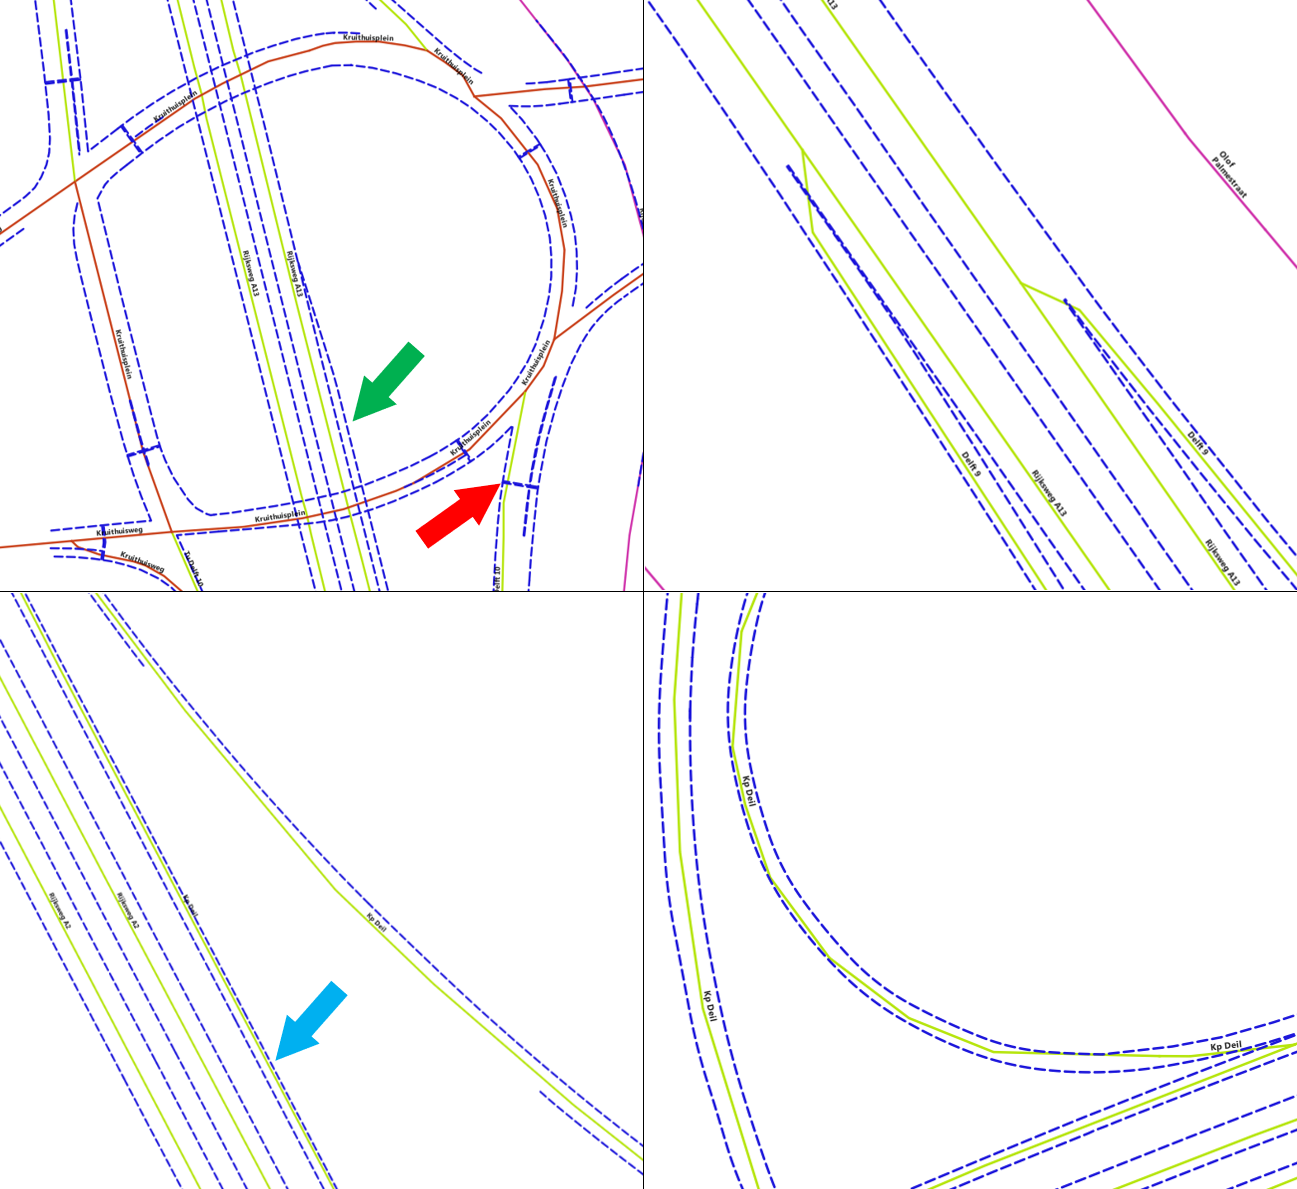
\includegraphics[width=0.95\linewidth]{final_report/figs/dtb_sample_07.png} 
    \caption{Renders of DTB \textit{verflijnen} overlaid with NWB centrelines, illustrating "compatibility issues" and individual DTB issues. NWB symbology is identical to the one used in \ref{fig:nwb}, blue dashed lines are the DTB lines. \textbf{Top left:} there is not necessarily only one \textit{verflijnen} line on either side of NWB (green arrow). Furthermore, stop lines are also often in this category. \textbf{Top right:} NWB motorway ramps often merge with the motorway lanes at unrealistic angles. This causes NWB to intersect DTB lines at these locations. \textbf{Bottom left:} DTB road edges are often missing. Furthermore, NWB centrelines may be very close to DTB edges, as indicated by the blue arrow. \textbf{Bottom right:} NWB discretisation and inaccuracy often results in angular lines in sharp bends. NWB often gets close to, even intersects DTB in such places. Although this is a 2D visualisation, DTB has 3D geometry as Figure \ref{fig:dtbahn} illustrates.}
    \label{fig:dtbnwb}
\end{figure}

\subsection{Digitaal Topografisch Bestand – DTB}
\label{sub:dtb}

\textit{[Subsection to be written.]}

\textit{[Content below copied from P2; to be adapted.]}

\begin{figure}[h!]
    \centering
    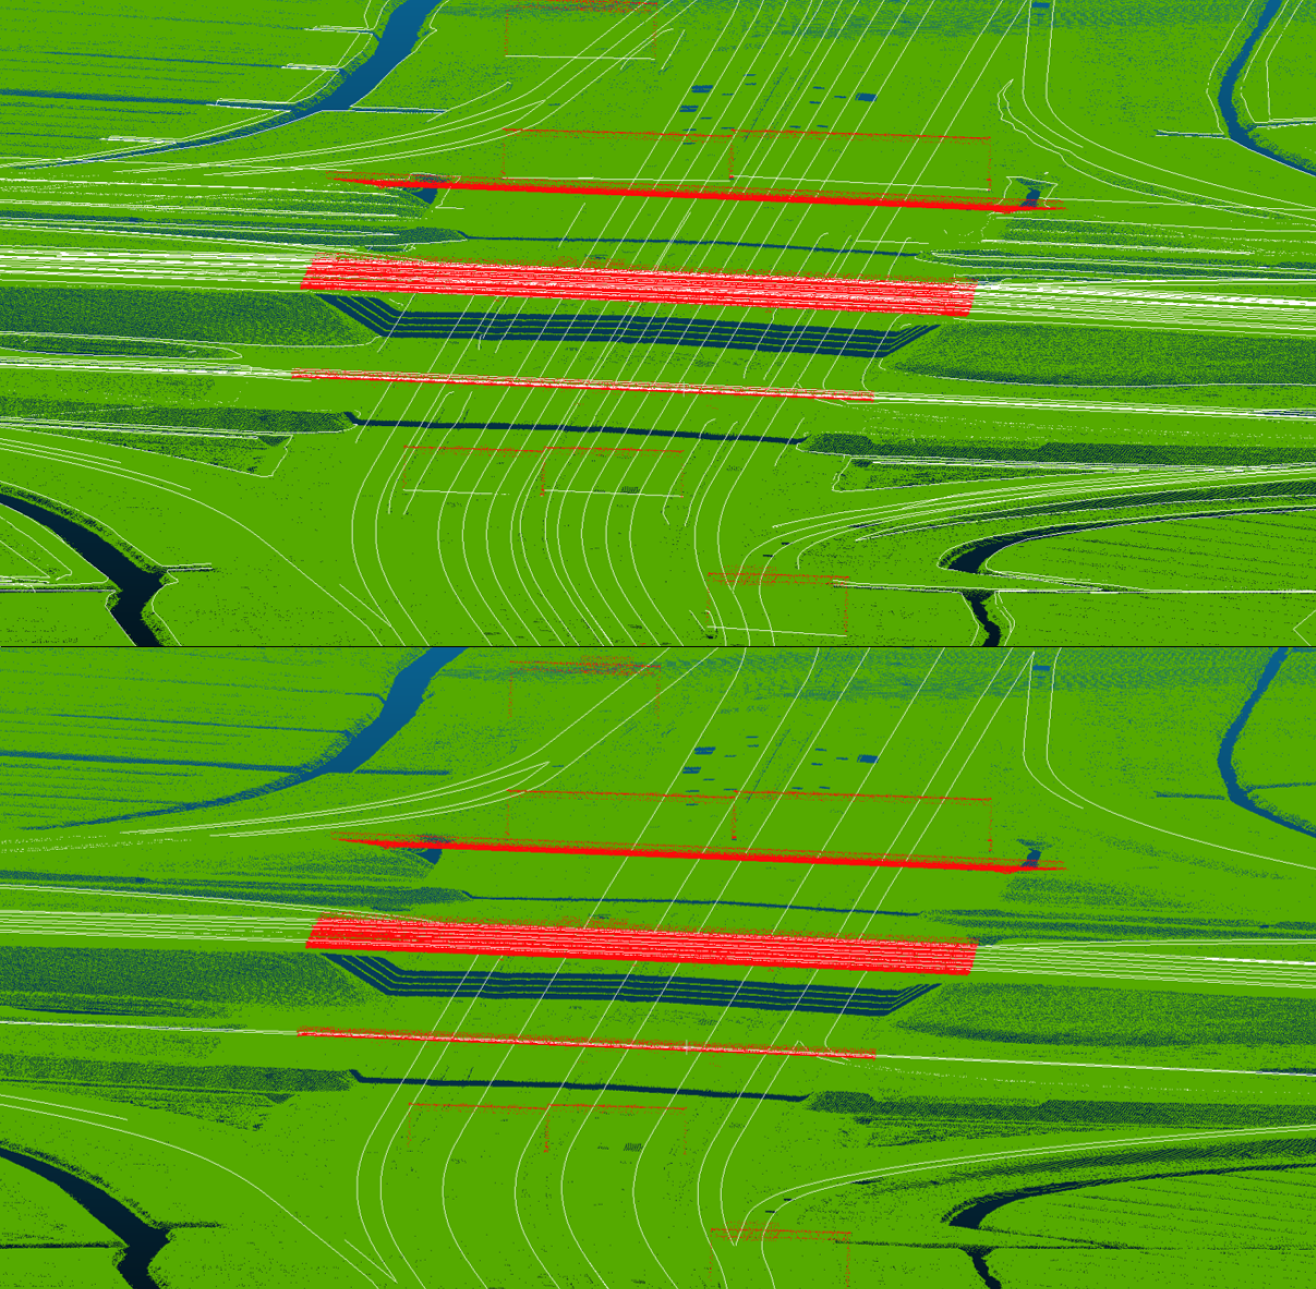
\includegraphics[width=0.95\linewidth]{final_report/figs/ahn_sample_10.png} 
    \caption{Renders of DTB line features overlain with AHN3 in 3D. Ground points are shown in green. \textbf{Top:} all DTB lines are shown, illustrating that other features, such as roadside slopes, canals, ditches, safety rails are represented in DTB. Full-width motorway signs are occasionally represented (either by lines on the road, or on the structure itself, inconsistently). \textbf{Bottom:} Only \textit{verflijnen} shown. The lines are generally in good agreement with AHN3 visually. This figure also illustrates that they may be useful for identifying which class-26 Lidar points lie on road surfaces, as they contain good first approximations for their elevations.}
    \label{fig:dtbahn}
\end{figure}

Like NWB, DTB (or more specifically, DTB-Droog, the DTB roads product) is a Dutch open data geospatial dataset in the \textit{ESRI Shapefile} format. For the purposes of this project, we only need DTB street outlines (edges), hence we can also regard this as a dataset comprised exclusively of \textit{MultiLineString} objects, making it identical to NWB in its data structure. DTB is managed by RWS and it is concerned only with state-owned roads and roads on state-leased land, which translate almost exclusively to NWB R-roads. DTB is, hence, not a reliable source of information about provincial roads (NWB P-roads), our other road type of interest. The DTB lines that are commonly used as road edges are not, in fact, the edges of the paved surface. They are called \textit{verflijnen}, and are the approximate locations of the painted lines representing the outermost edges of the area open to traffic. This is a lucky correspondence with NWB, as it too, contains the centrelines of the areas of roads that are open to traffic. The second-best option would be to use the category \textit{gelederail constructie}, which generally provide good approximations of the edges of the paved surfaces on which the \textit{verflijnen} were painted. Unfortunately, these correspond to the location of safety rails, and as such they are sometimes not on the road and are also not always present. Like NWB (but unlike AHN), DTB’s acquisition also concerns several organisations performing various types of sensing, which are then semi-automatically assembled into the complete DTB product. DTB lines are primarily photogrammetry-derived, with land-based surveying methods and car-mounted Lidar (MLS) used in some areas to improve accuracy (\cite{oudeElberink_vosselman_2012}). The documentation of DTB consist of a documentation (\cite{dtb_docs}) and a handbook (\cite{dtb_handbook}). The accuracy of DTB is not published by RWS or any other organisation contributing to or using the dataset, although it is generally thought to be quite accurate. It is mostly used for purposes relating to road management and civil engineering and apart from road edges, it contains more than 400 other types of semantically identified roadside object types. As most users of DTB work in GIS environments, particular care is taken to separate objects into layers in such a way that inside any one layer, they never overlap. This means that they can be processed using 2D GIS tools easier, reducing the significance of elevation to a mere semantic detail (non-geometric attribute). Whenever objects in any given such layer are found in the same position (or closer than a certain threshold), they are automatically shifted by a maximum distance of 5 centimetres to eliminate the overlap, most commonly for DTB road signs. While descriptions in the documentation can be found suggesting that DTB lines are measured accurately, I must consider the formal accuracy of DTB unknown due to the lack of any numerical figures or other evidence to support this. Furthermore, as I illustrate in \ref{fig:dtbnwb}, a visual comparison with NWB reveals various types of significant inconsistencies and interpretation issues. A visual comparison with AHN3 is also shown in \ref{fig:dtbahn}.

\section{Methods of existing implementations}
\label{sec:methodsexisting}

\subsection{NDW prototype}
\label{sub:ndwprototype}

\textit{[Subsection to be written.]}

\textit{[Content below copied from P2; to be adapted.]}

NDW themselves produced a non-commercial prototype implementation, which can achieve a 3D enrichment of NWB with only a few gaps in the produced elevation profiles. Although their workflow does not have a formal documentation, I have been given a verbal description of it, as well as the output. Based on my understanding of these, their primary technique involved snapping close-by AHN3 Lidar points to the line geometries of NWB. Notable problems with the implementation included non-road points being snapped to centrelines, causing road centrelines to be given overestimated elevations, in turn resulting in sudden jumps in the elevation profiles. Furthermore, no close-by points could be found for underground roads (i.e. tunnels), and strongly occluded parts of roads. For small gaps, this was resolved partially by writing an algorithm to interpolate linearly inside NWB, using the closest vertices where snapping was successful. For larger gaps, an attempt was made to resolve issues by including information from external sources semi-automatically. Neither issue could be fully resolved via these approaches, hence the results of this project were only used by NDW to gain a better understanding of the problem and the expected challanges. For a reliable, commercial toolbox they subsequently commissioned an implementation from RHDHV.

\subsection{RHDHV commercial toolbox}
\label{sub:commercialproduct}

\subsubsection{Overview of commercial methods}

\textit{[Subsubsection to be written.]}

\textit{[Content below copied from P2; to be adapted.]}

RHDHV developed their implementation in parallel with the \textit{planning} of the present scientific research. I have attended NDW-RHDHV meetings, discussed the implementation directly with RHDHV, and was granted access to the codebase of the project. Understanding their implementation is crucial for this research, as it aims to both assess the accuracy of the commercial implementation, as well as in part base its methodology and implementation on the suspected shortcomings of the commercial implementation. The steps of the procedure are briefly described below.

First, where NWB vertices are too sparse, densification takes place; additional temporary vertices are created inside NWB line segments. Then, \textit{different} workflows are initiated for R-roads and P-roads.

For P-roads (for which DTB data does not generally exist), the workflow is conceptually similar to the one in the prototype, with the notable difference of using AHN3 DTM rasters rather than the point cloud. Because AHN3 DTM rasters are badly affected by both large holes and small groups of missing pixels (due to the fixed-parameter IDW interpolation that was used to generate them), RHDHV could only make use of them by filling in the gaps of the raster using linear interpolation in a 3D TIN created from extruded raster pixel centres. They overlaid the raster tiles with NWB vertices (including the dense, temporary vertices) and interpolated their elevations using bilinear interpolation inside the raster.

\begin{figure}[h]
    \centering
    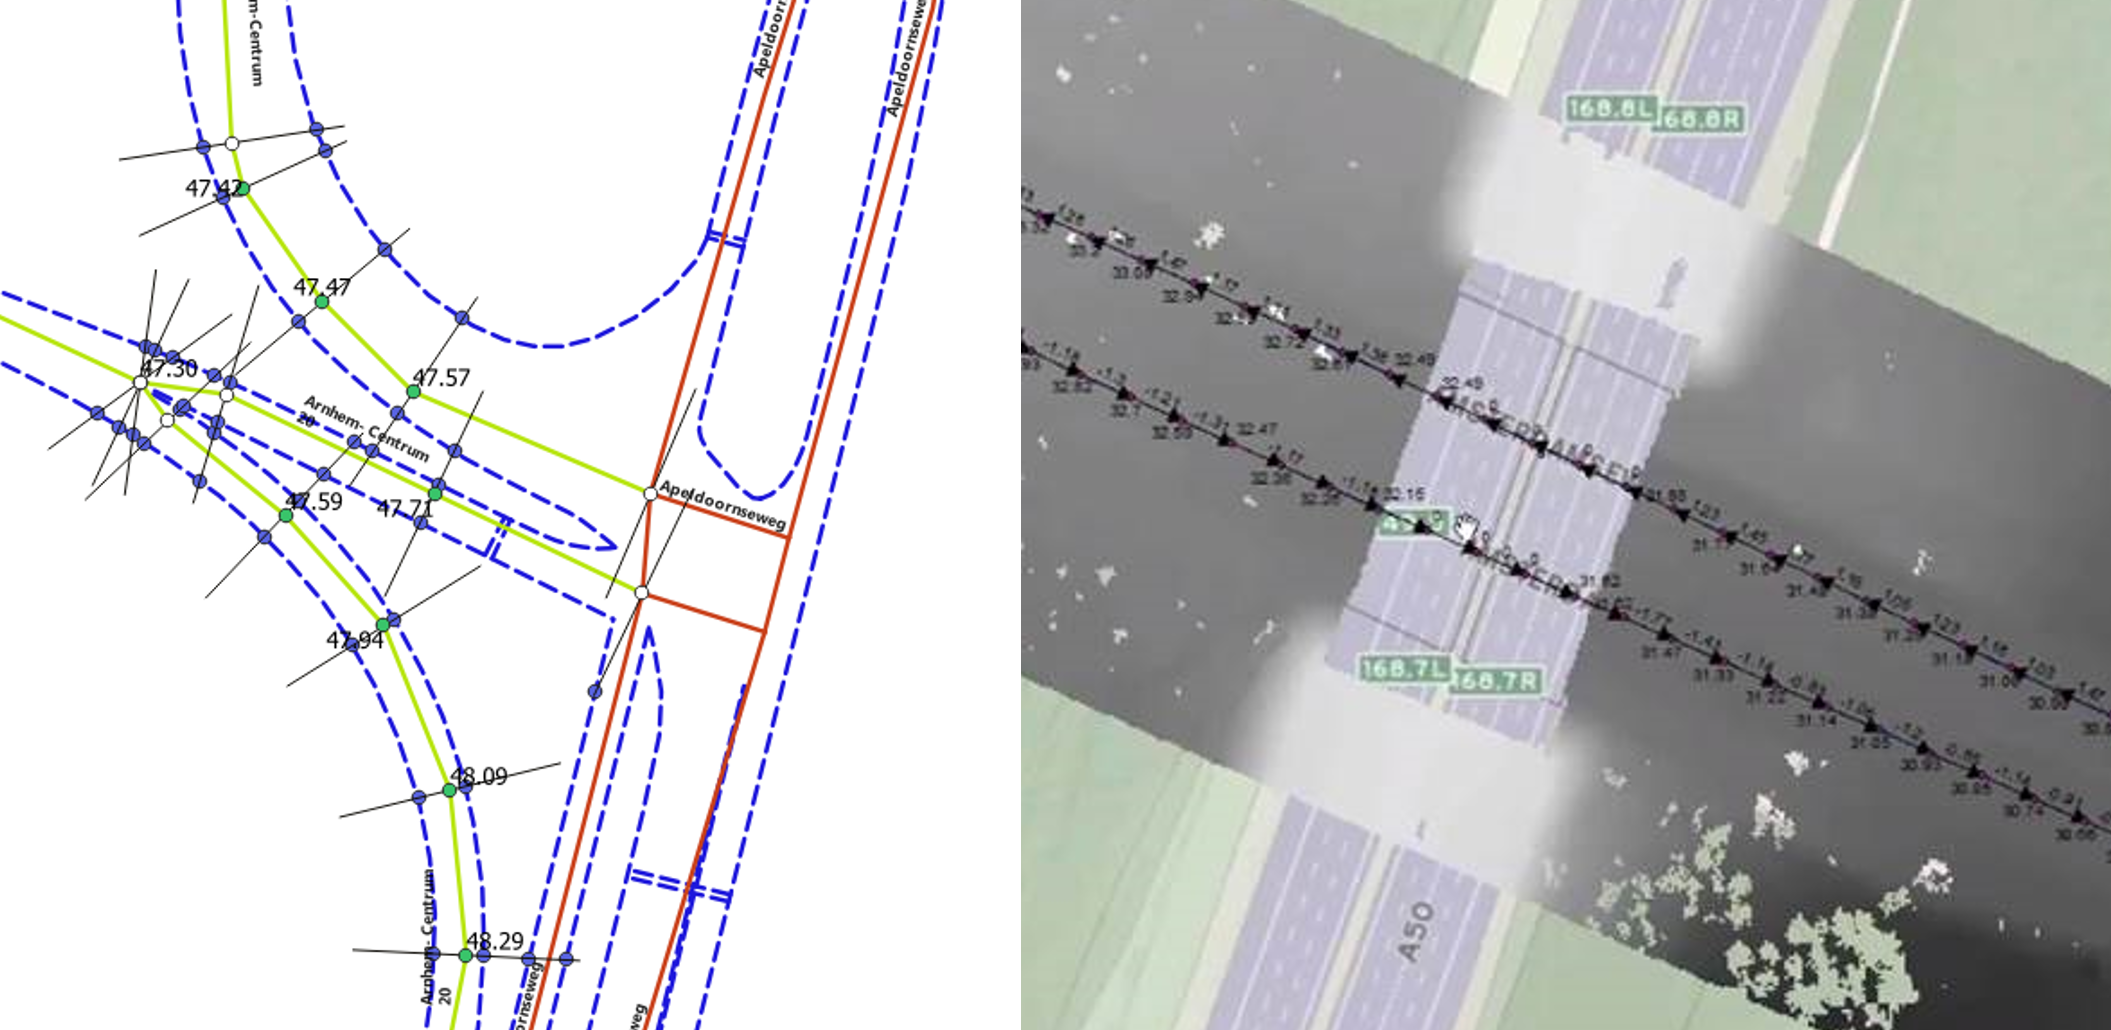
\includegraphics[width=\linewidth]{final_report/figs/rhdhv_combined.png}
    \caption{Illustrations of RHDHV's commercial implementation. \textbf{Left:} The cross-sections that are constructed on NWB vertices are shown as black lines. Green circles denote those vertices where the cross section could be properly intersected with DTB \textit{verflijnen} (blue circles) and thus be given an elevation value. White circles denote where the procedure failed, and AHN raster-based interpolation was necessary. This render illustrates that in sharp bends (where the cross-section might not intersect DTB orthogonally) and close to intersections, this workflow often fails, and that P-roads are not processed in this way (they have DTB edges in this particular location only because they are close to R-roads). \textbf{Right:} AHN-based interpolation is used for P-roads, and as a fallback mechanism where DTB-based interpolation fails. The rasters are overlain with NWB to yield elevation values, and as the DSM rasters contain holes, they are patched in by pre-interpolating them before this step. In this illustration, the holes are left in to show that two types of holes generally occur: small-scale ones due to objects such as street furniture, vehicles and vegetation, and large ones that are typically due to occlusion from overlapping buildings or bridges (as in this case). The test build shown here uses AHN2 rasters.}
    \label{fig:rhdhv}
\end{figure}

For R-roads DTB is available, and the assumption is made by RHDHV that it is more accurate than AHN3 (or at least the stock DTM tiles generated from AHN3), to the extent where it should be the primary source of elevation data. Priority is thus always given to it in the procedure, with AHN-based interpolation used only as a fallback mechanism in case DTB-based height estimation fails. The goal of the procedure is to find the DTB line segments that delineate the road edges at any given location in the NWB and deduce elevations from them. First, 2D cross-sections are constructed on NWB vertices, with each given the mean azimuth of the two NWB line segments that they are part of, and also on densified vertices, which receive azimuth values based simply on the azimuth of their parent line segments. DTB lines are then intersected with the cross-sections and for each cross-section, the closest DTB line that satisfies a relative angle condition is picked on both sides. Elevation is then first linearly interpolated inside the two chosen DTB segments to yield values exactly at their intersections with the cross-section. Then, elevation is interpolated linearly along the cross-section itself to yield the final elevation of the NWB vertex or densified temporary vertex.

The angle condition mentioned above is a threshold-based evaluation concerning the angle between intersected DTB lines and cross-sections, and is intended to ensure that the chosen DTB segment indeed represents the edge of the selected road, rather than some other feature, or the edge of another road. Hence, the assumption is made that the DTB line segments representing road edges are roughly parallel with the relevant NWB centrelines and lie close to them. Implicitly, this also assumes that NWB centrelines will lie between DTB road edges. In practice, these assumptions are not valid in general, hence a range of failsafe mechanisms needed to be implemented. Wherever the algorithm only finds a suitable DTB intersection on \textit{one} side of NWB, it is only that side from which the elevation value is deduced. If no suitable intersection can be found whatsoever, the AHN3 raster-based interpolation is used instead. At NWB centreline end vertices (where no intersection exists, i.e. dead ends), the previous vertex’s elevation is simply repeated. The described methodology is illustrated in Figure \ref{fig:rhdhv}.

It is worth mentioning that the RHDHV implementation deals with all non-standard input data sets (i.e. small-scale engineering models, road management datasets, etc.) by first converting them to rasters with the same specifications as AHN3 DTM tiles and mosaicking them into an output raster based on a priority list, before filling in any remaining gaps and interpolating bilinearly.

\subsubsection{Potential limitations}

\textit{[Subsubsection to be written.]}

\textit{[Content below copied from P2; to be adapted.]}

From a scientific point of view, there are numerous potential issues suggested by the description of this workflow. For instance, point cloud to raster conversion is, by definition, associated with inherent information loss (less raster cells than pixels), and further reduction in accuracy is introduced by the interpolation mechanism itself. Radial IDW was used to generate AHN3 DTM tiles, which several of the reviewed papers found to be specifically unsuitable for interpolating large-scale areas in which zones of decreased point density or gaps exist – both of which characterise ground-filtered AHN data (e.g. \cite{guo_etal_2010}). In addition, the procedure performs another layer of interpolation to infill gaps, which may further deteriorate accuracy. Furthermore, RHDHV uses bilinear interpolation inside the raster to produce NWB elevations, which is suggested by \cite{shi_etal_2005}, to be less accurate than other common methods such as bicubic. In terms of their strong prioritising of DTB for R-roads, I should remark that DTB itself is also a secondary source of information (it is based on a procedural combination of data from various types of sensing, into vector features), and in contrast with AHN3, neither its overall nor its local accuracy are known. While it no doubt contains valuable information, relying on it as the sole source of elevation data does not appear to permit the estimation of output accuracy, which is a pre-requisite of compliance with SWUNG2.

Care will be taken to examine how the same challenges as we expect to face regarding output accuracy and 3D road interactions are handled by the commercial implementation – in fact, some of my research questions are based specifically on challanges reported by the developers of the commercial implementation, and the known shortcomings of their final product. Our preliminary analysis of the implementation indicates that for instance, it uses input data with non-validated accuracy for motorways, and simple bilinear interpolation in poorly interpolated, Lidar-based raster DTMs for provincial roads. Furthermore, it only handles 3D interactions explicitly for motorways and even for these, it does so via a series of assumptions that do not hold in general, necessitating the use of various fallback mechanisms. This comparison may provide an insight into some aspects of 3D geospatial data processing that are frequently overlooked, or oversimplified in commercial implementations.